\section{Vibração induzida por vórtices em vãos livres}\label{chap:viv}

Quando um fluido de baixa viscosidade encontra um obstáculo, forma-se uma camada limite.
Esta fina camada de fluido está sujeita aos efeitos das forças viscosas.
Nesta camada, a velocidade do fluxo varia rapidamente, ficando cada vez mais lenta, formando um escoamento rotacional dentro da camada limite.
Para determinadas velocidades de escoamento, a camada limite se desprende do obstáculo, formando uma esteira de vórtices, conhecida como esteira de von Kármán~\cite{Currie2002}, conforme visto na Figura~\ref{fig:viv_shading}.
Como consequência direta do desprendimento de vórtices, surge uma força oscilatória transversal ao fluxo, que age sobre o obstáculo, resultando em oscilações verticais e horizontais~\cite{Nielsen2002}.

\begin{figure}[!ht]
    \centering
    \caption{Esteira de Von Kármán.}\label{fig:viv_shading}
    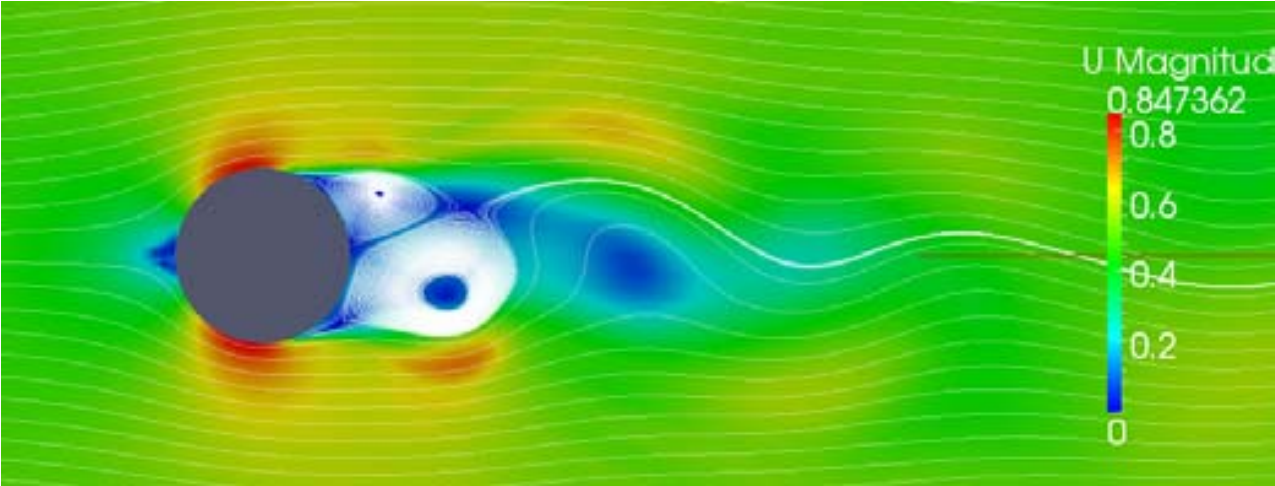
\includegraphics[width=0.6\textwidth]{imagens/viv_shading}
    \fonte{\citeonline{VandenAbeele2013}}
\end{figure}

A frequência do desprendimento de vórtices causado por um fluxo normal ao obstáculo (o duto em vão livre, no caso em questão), é governado pelo número de Strouhal, diâmetro externo e velocidade de fluxo~\cite{Mork2003}.
O número de Strouhal pode ser obtido pela expressão
\begin{equation}
    S_t = (f L) / V
\end{equation}
onde $f$ é a frequência de vórtices, $L$ é o comprimento característico e $V$ é a velocidade do fluxo.
Quando a velocidade do fluxo alcança uma das frequências naturais da estrutura, ela começa a vibrar e estas duas vibrações se correlacionam, causando vibrações de grande amplitude e grande dano (\textit{lock-in})~\cite{Mork2003}.

Como os dutos são geralmente modelados como cilindros, é importante entender como funciona o comportamento do fluxo de fluido ao redor dessa estrutura. Segundo \apudonline{Sumer1995}{Batchelor1967}, ao estudar vibrações de cilindros em corrente constante, inicia-se o desprendimento de vórtices quando o número de Reynolds,
\begin{equation}
    R_e = (U D)/\nu
\end{equation}
é maior que $40$, onde $U$ é a velocidade do fluxo, $D$ é o diâmetro do cilindro e $\nu$ é a viscosidade cinemática~\cite{Sumer1995}.

O desprendimento de vórtices induz uma variação cíclica de forças no cilindro.
Assim, enquanto uma força de sustentação (\textit{lift force}) oscila à mesma frequência do desprendimento de vórtices, a força de arrasto (\textit{drag force}) oscila à duas vezes esta mesma frequência~\cite{Sumer1995}.
Essas forças oscilatórias, os vórtices, podem induzir vibrações na direção ortogonal ao fluxo, \textit{cross-flow} (CF), e na direção do fluxo, \textit{in-line} (IL), denominadas vibrações induzidas por vórtices (VIV).

Os diversos dutos submarinos, que tem como objetivo o transporte de fluidos, seja entre o poço e a plataforma, entre plataformas, etc., estão sujeitos ao fluxo intermitente de cargas ambientais.
Essas cargas tornam-se um desafio ainda maior quando os dutos, instalados diretamente no irregular leito marinho, encontram-se em vãos livres~\cite{Fyrileiv1998}, como ilustrado na~\autoref{fig:freespan}.

\begin{figure}[!ht]
	\centering
    \caption{Duto em Vão livre e direções das oscilações.}\label{fig:freespan}
	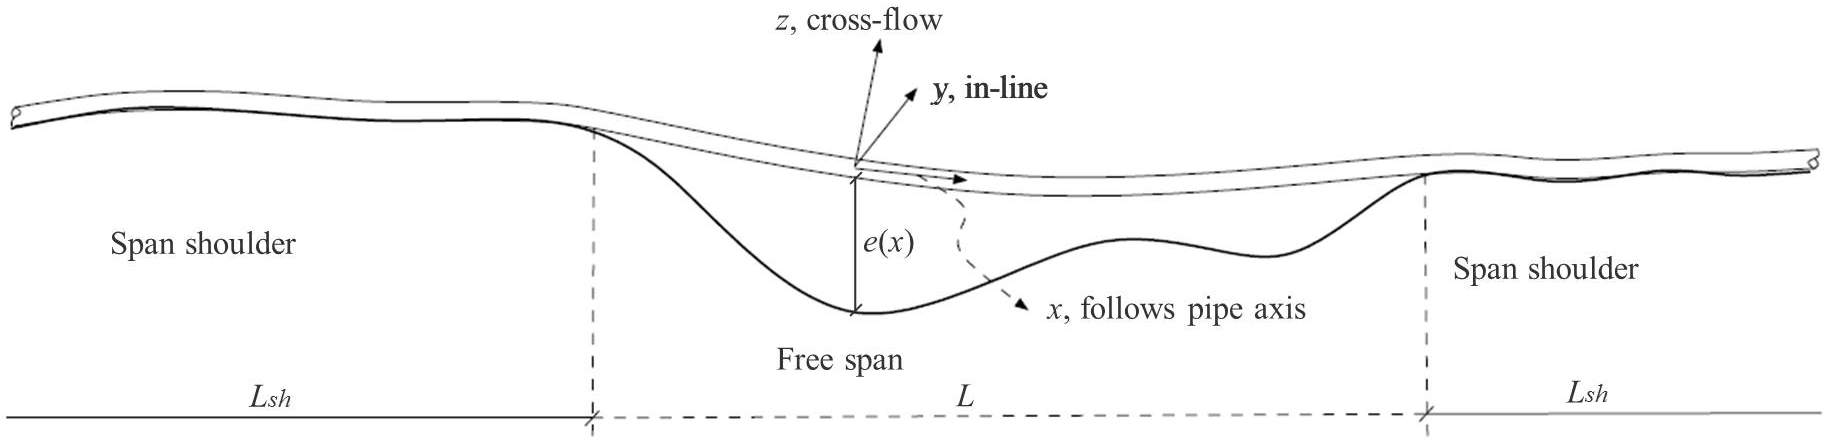
\includegraphics[width=1\textwidth]{imagens/freespan}
    \fonte{Adaptado de \citeonline{DNV2017}}
\end{figure}

Vãos livres não aparecem apenas quando os dutos são instalados em leito irregular, mas também quando ocorre erosão posterior (\textit{scouring}\footnote{Erosão do solo marinho causada pela ação de ondas ou correntes. Caracteriza-se pela remoção de sedimentos com formação de cavidades ou canais.}), devido, por exemplo, a suportes artificiais.
Com o duto exposto às ondas e correntes, a parte não apoiada estará suscetível à VIV.\@
Caso a frequência de desprendimento alcance uma das frequências naturais do duto, esse poderá entrar em ressonância.
As excitações dinâmicas podem causar danos por fadiga, sendo importante identificar os corretos procedimentos de intervenção, seja no duto ou no leito marinho.

A \dnvf105 é uma referência técnica adotada mundialmente no estudo de dutos em vão livre.
Nele está presente uma metodologia baseada em modelos de resposta a fim de avaliar a fadiga causada por VIV\@.
Estes modelos representam relações empíricas entre a velocidade reduzida (\autoref{eq:viv-Vr}) e a amplitude de resposta adimensional, utilizadas para prever as amplitudes de vibração nas direções \textit{in-line} e \textit{cross-flow}~\cite{Mork2003,DNV2017}.
Além desta, a recomendação prática sugere também um método baseado no coeficiente de sustentação e nas curvas do coeficiente de massa adicional como função da amplitude de resposta adimensional e da frequência de vibração adimensional~\cite{DNV2017}.
Como terceira opção, a \dnvf105 indica o uso de fluidodinâmica computacional (CFD, na sigla em inglês) para escoamento turbulento ao redor dos dutos para avaliação do VIV\@.

A \dnvf105 considera dois modelos para estimar a resposta dinâmica em um vão livre: Modelo de Resposta (\textit{Response Model}--RM) e Modelo de Força (\textit{Force Model}--FM).
A escolha do modelo, segundo~\citeonline{Tura1994}, depende: (i) do comportamento dos carregamentos ambientais, isto é, quando há ressonância induzida por vórtice, aplica-se RM\@; e quando o comportamento do vão livre é afetado por carregamentos periódicos com pouca ou nenhuma amplificação dinâmica, aplica-se FM\@; (ii) da direção e tipo de fluxo, RM é aplicável na direção \textit{in-line} para corrente contínua e na direção \textit{cross-flow} para qualquer padrão de fluxo; o FM é aplicado na direção \textit{in-line} para carregamentos de onda direto.

A \dnvf105 pode ser aplicada para vãos únicos e múltiplos onde um modo de vibração é predominante (\textit{single-mode}), conforme a \autoref{fig:vaos_tipicos}.
Porém, a combinação de vãos de grande extensão e altas correntes, ou ainda vãos múltiplos, faz com que não apenas os modos fundamentais sejam ativados, mas também diversos outros modos de ordem mais alta (\textit{multi-mode}).

\begin{figure}[!ht]
	\centering
    \caption{Configurações típicas para vãos.}\label{fig:vaos_tipicos}
	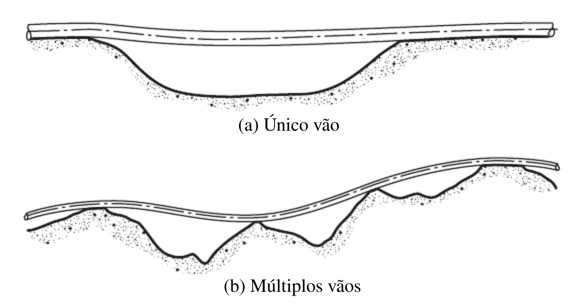
\includegraphics[width=0.7\textwidth]{imagens/vaos_tipicos}
    \fonte{Adaptado de \citeonline{Bai2014}}
\end{figure}


\subsection{Modelos de respostas}

Os modelos de resposta relacionam a velocidade do fluxo do flúido externo e a amplitude de vibração do duto em casa direção (\textit{in-line} e \textit{cross-flow}). Estes modelos pode então ser construído através do conjunto de equações que dependem principalmente da velocidade reduzida $V_R$ e do ângulo do fluxo $\theta_\mathit{rel}$.

Segundo a \dnvf105 o fluxo pode ser dividido em duas zonas: (i) uma zona exterior, distante do solo marinho, onde velocidade de corrente média e a turbulência variam muito pouco na direção horizontal, e (ii) uma zona interior, onde a velocidade de corrente média e a turbulência têm variações consideráveis na direção horizontal. Uma vez que as medições da corrente são realizadas na zona exterior, fora da camada limite, a velocidade de corrente $U_c$ no duto pode ser aproximada a partir da equação
\begin{equation}
\label{eq:vel-corrente}
U_c = R_c U(z_r) \frac{\ln{(e+D/2)} - \ln(z_0)}{\ln (z_r)- \ln (z_0)},
\end{equation}
em que $U(z_r)$ é a velocidade da corrente na altura de referência $z_r$, $e$ é o gap entre o duto e solo, $z_0$ é a cota de referência e $D$ é o diâmetro externo do duto.

Uma vez encontrada a velocidade da corrente na zona interior, isto é, próxima do solo, a velocidade reduzida $V_R$ pode ser calculada assim
\begin{equation}
\label{eq:viv-Vr}
V_R = \frac{U_c + U_w}{f_n D},
\end{equation}
onde $U_w$ é a velocidade de fluxo induzida por onda e $f_n$ é a frequência natural de amplitude.

O parâmetro de estabilidade $K_S$, representa o amortecimento para uma dada forma modal, sendo obtido a partir da equação
\begin{equation}
\label{eq:viv-Ks}
K_S = \frac{4 \pi m_e \zeta_T}{\rho_w D^2},
\end{equation}
em que $\rho_w$ é a densidade da água e $\zeta_T$ é a taxa de amortecimento modal total.

Com esses valores calculados, e pode-se construir a curva que relaciona velocidade reduzida e amplitude de vibração \textit{in-line} para diâmetro unitário, semelhante a \autoref{fig:viv-responsemodelil}, onde as coordenadas dos pontos são dados nas equações do ítem 4.6.4 da \dnvf105.

\begin{figure}[!ht]
    \centering
    \caption{Curva de modelo de resposta \textit{in-line}.}\label{fig:viv-responsemodelil}
    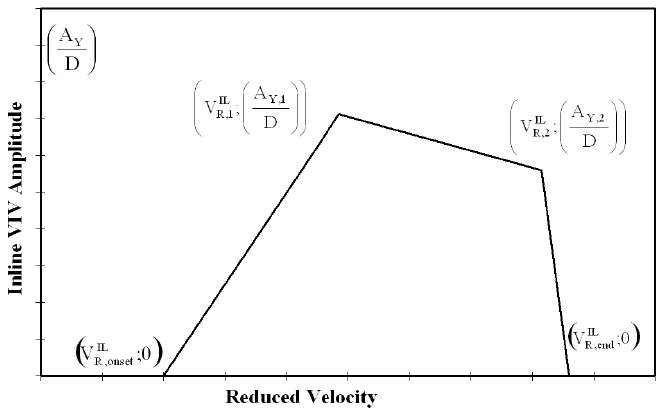
\includegraphics[width=0.65\linewidth]{imagens/response_model_IL}
    \fonte{Adaptado de \citeonline{DNV2017}}
\end{figure}

Conforme observado na \dnvf105, a resposta de amplitude de um duto vibrando na direção \textit{in-line}, contempla regiões com velocidade de corrente entre 1,0 e 4,5.
Tem-se então que a resposta na direção longitudinal depende dos parâmetros de velocidade de corrente, estabilidade, intensidade de turbulência e do ângulo entre a corrente e o duto.
Percebe-se que, à medida que o parâmetro de estabilidade aumenta, a amplitude de resposta tende à diminuir, uma vez que este é proporcional ao amortecimento do sistema~(\autoref{eq:viv-Ks}).

Para o modelo de resposta \textit{cross-flow} também  é necessário calcular alguns outros parâmetros. Dessa vez, inicia-se com o cálculo do fator de correção para considerar a proximidade do duto com o solo
\begin{equation}
\label{eq:viv-Psi}
\Psi_{\mathit{proxi}, \mathit{onset}} =
\begin{cases}
\frac{1}{5}\left(4 + 1,25\frac{e}{D} \right) & \mathrm{para}~\frac{e}{D} < 0,8\\
1                                            & \mathrm{caso~contr\acute{a}rio}
\end{cases}
\end{equation}

Caso o duto esteja localizado próximo ou em trincheiras é necessário considerar o fator de correção específico
\begin{equation}
\label{eq:viv-Psitren}
\Psi_{\mathit{trench}, \mathit{onset}} = 1 + 0,5\frac{\Delta}{D}
\end{equation}
onde $\Delta$ é a profundidade da trincheira.

Com esses valores calculados, pode-se construir a curva que relaciona velocidade reduzida e amplitude de vibração para diâmetro unitário, semelhante a \autoref{fig:viv-responsemodelcf}, onde as coordenadas dos pontos são dados nas equações do ítem 4.6.4 da \dnvf105.

\begin{figure}[!ht]
    \centering
    \caption{Curva de modelo de resposta \textit{cross-flow}.}\label{fig:viv-responsemodelcf}
    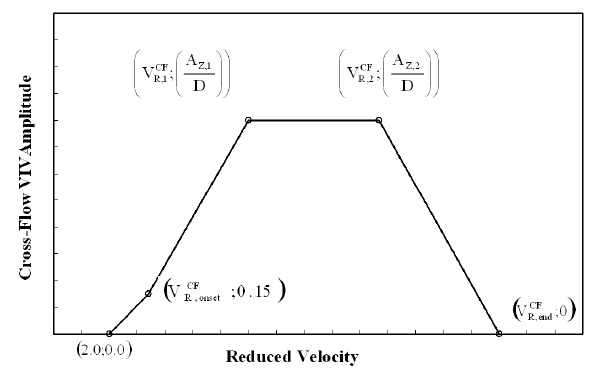
\includegraphics[width=0.65\linewidth]{imagens/response_model_CF}
    \fonte{Adaptado de \citeonline{DNV2017}}
\end{figure}


\subsection{\label{sec:multimode}Resposta \textit{multi-mode}}


A resposta do vão livre pode ser dada em função de uma coordenada $x$ ao longo da direção longitudinal do duto.
Para cada combinação relevante de estado de mar e velocidade de corrente, um número de modos pode ser excitado simultaneamente na mesma direção, dando origem a uma resposta \textit{multi-mode}.
Todavia, o número de modos que responderão e o quanto cada modo contribuirá para o dano por fadiga dependerá da velocidade do fluxo, da posição no eixo $x$ e da competição com outros modos.

A \dnvf105 define três diferentes tipos de modos:
\begin{description}
	\item[Modos ativos] são os modos que podem ser excitados por VIV\@. Com base no itém 2.3.3 da DNVGL-RP-F105, os critério de definição para que um modo \textit{in-line} com frequência $f_{IL,j}$, ou \textit{cross-flow} com frequência $f_{CF,j}$, seja considerado ativo é:

    \begin{equation}
        \begin{aligned}
        f_{I L, j} & \leq \frac{U_{extreme} \gamma_{f,IL}}{V_{R,\text{onset}}^{IL} D} \\
        f_{C F, j} & \leq \frac{U_{extreme} \gamma_{f,CF}}{2D}
        \end{aligned}
    \end{equation}
    sendo $\gamma_{f,IL}$ e $\gamma_{f,CF}$ coeficientes de segurança, variando de 1 a 1,3 a depender da classe de segurança e nível de
    definição do vão livre (item 2.7.2 da DNVGL-RP-F105). Já $U_{extreme}$ é a velocidade do fluxo perpendicular ao duto que considera velocidades de corrente e onda, e pode considerar combinações de períodos de retorno de 1, 10 e 100 anos.
    Um modo que não passível de ativação pode ser totalmente desconsiderado nas análises em todos os pontos e velocidades de fluxo.

    \item[Modos participantes] são modos ativos que têm amplitude de tensão relevante em um, ou ambos os lados, de um ponto na coordenada $x$ ao longo do duto. Para que um modo $j$ seja considerado participante no vão, é necessário que a seguinte condição (presente no item 4.3.3) seja atendida:
    \[
    \left|A_{\textbf{IL/CF}, j}(x)\right| \geq \frac{A_{IL/CF}^{\max}}{10} \text{ para algum } x \in (x_{\text{start},j}, x_{\text{end}, j})
    \]
    sendo
    \[
    A_{IL/CF, j}(x) = (1+CSF) D \kappa_{j}(x) E r
    \]
    onde

    \begin{tabular}{rl}
        $\mathit{CSF}$                            & fator de rigidez do concreto\\
        $\kappa_{j}(x)$                           & curvatura do modo na posição $x$\\
        $E$                                       & módulo de elasticidade\\
        $r$                                       & coordenada radial da seção transversal do duto\\
        $(x_{\text{start},j}, x_{\text{end}, j})$ & intervalo de influência do modo
    \end{tabular}

	\item [Modos contribuintes] são modos participantes que deve satisfizer um dos seguintes critérios:

        \begin{itemize}
    	\item direção \textit{cross-flow}: ${(A_Z/D)}_j \geq 0,1{(A_Z/D)}_{\max}$

        \item direção \textit{in-line}: $S_{\mathit{IL}, \mathit{j}}^{P}(x) \geq 0,1 S_\mathit{IL}^{\max}(x)$
        \end{itemize}

	onde ${(A_Z/D)}_j$ é a amplitude VIV normalizada para o j-ésimo modo, ${(A_Z/D)}_{\max}$ é a amplitude VIV normalizada para o modo \textit{cross-flow}  dominante, $S_{\mathit{IL}, \mathit{j}}^{P}(x)$ é a amplitude de tensões de reposta preliminar para o j-ésimo modo \textit{in-line} e $S_\mathit{IL}^{\max}(x)$ é a amplitude de tensões de resposta associadas ao modo \textit{in-line} dominante.

\end{description}

Baseado nos modelos de resposta \textit{single-mode}, pode-se calcular as amplitudes do VIV para todos os modos (\autoref{procedure_il}).
Assim, precisamos calcular VIV \textit{cross-flow} e \textit{in-line} para cada velocidade de corrente, estado de mar e em cada ponto com se os seguintes procedimentos:

\begin{itemize}

\item VIV \textit{cross-flow}\label{procedure_il}

\begin{enumerate}
\item Identifica-se todos os modos participantes (\textit{single} ou \textit{multi location})

\item Com o modelo de resposta \textit{cross-flow}:
	\begin{enumerate}
    \item Calcula-se a amplitude VIV normalizada para cada modo ${(A_Z/D)}_j$

	\item Identifica-se o modo dominante, isto é, ${(A_Z/D)}_{\max}$

    \item Identificam-se os modos fracos $0,1{(A_Z/D)}_{\max} \leq {(A_Z/D)}_j \leq {(A_Z/D)}_{\max}$

    \item Desconsidera-se os modos irrelevantes: ${(A_Z/D)}_j$ < $0,1{(A_Z/D)}_{\max}$
    \end{enumerate}

\item Usando o modelo de resposta para baixos valores de Keulegan-Carpenter (\textit{low Keulegan Carpenter flow regime}--LKCR), calcula-se ${(A_Z/D)}_j$ para cada modo.

\item Determina-se a resposta de tensão combinada:
    \[
    S_{\mathit{comb}, \mathit{CF}} = \max\left( S_{\mathit{comb}, \mathit{CF}}^\mathit{RM} ~,~ S_{\mathit{comb}, \mathit{CF}}^\mathit{LKCR} \right)
    \]

\item Determina-se a frequência de contagem de ciclos.

\end{enumerate}

\item VIV \textit{in-line}

\begin{enumerate}
    \item Identifica-se todos os modos participantes (\textit{single} ou \textit{multi location})

    \item Com o modelo de resposta \textit{in-line}:

    \begin{enumerate}
    	\item Calcula-se a amplitude VIV normalizada para cada modo ${(A_Y/D)}_j$

    	\item Identifica-se o modo dominante, isto é, o modo com $S_\mathit{IL}^{\max}(x)$

    	\item Identificam-se potenciais modos fracos: $0,1 S_\mathit{IL}^{\max}(x) \leq S_{\mathit{IL}, \mathit{j}}^{P}(x) \leq S_\mathit{IL}^{\max}(x)$

    	\item Desconsideram-se os modos irrelevantes: $S_{\mathit{IL}, \mathit{j}}^{P}(x) < 0,1 S_\mathit{IL}^{\max}(x)$
    \end{enumerate}

        \item Reduzir os modos fracos.
        Para VIV \textit{in-line}, dois modos adjacentes podem competir se suas frequências forem próximas, ou agir de forma independente se estiverem distantes.
        A \dnvf105 define que os modos competem se a razão entre as frequências é menor que 2, isto é, $\frac{f_\mathit{n+1}}{f_n} < 2$.
        Em modos que estão competindo, considera-se que apenas o ``vencedor'' da competição (maior valor de $S_{\mathit{IL}}^{P}(x)$) pode ter máxima amplificação, enquanto a amplificação do modo ``perdedor'' é reduzida à metade. É interessante ressaltar que modos que não competem não têm redução.

        \item Calcular o intervalo de tensões \textit{in-line} excitados pelo modo \textit{cross-flow} dominante $S_{\mathit{\textit{cross-flow}}-\mathit{IL}}(x)$.

        Para cada ponto e cada modo, calcula-se o intervalo de tensões induzido por VIV \textit{in-line} para os modos contribuintes:
            \[S_{\mathit{IL}, \mathit{j}}^\mathit{RM}(x) = S_{\mathit{IL}, \mathit{j}}^{P} \cdot 0,5^{\beta_j (x)}\]

        Assume-se que apenas o modo \textit{cross-flow} dominante é capaz de contribuir para o movimento \textit{in-line} induzido pelo modo transversal.
        Desta forma, o modo \textit{in-line} participante cuja frequência natural é próxima a duas vezes a resposta \textit{cross-flow} dominante é escolhido como candidato a VIV \textit{in-line} induzido por \textit{cross-flow}.

        A amplitude de tensões \textit{in-line} excitados pelo modo \textit{cross-flow} dominante é dado por:

       	    \[S_{\mathit{CF-IL}}(x) = 0,8 \cdot A_{\mathit{IL}, \mathit{k}}~(x) \cdot {\left(\frac{A_{z}}{D}\right)}_{\max}~\cdot~R_k \cdot \gamma_s\]

        \item  Escolher o maior $S_\mathit{IL}^\mathit{RM}(x)$ e $S_{\mathit{CF-IL}}(x)$ para cada modo;

        \item Determinar a faixa de resposta de tensão combinada e a frequência de contagem de ciclos.
    \end{enumerate}

\end{itemize}
